%%%%%%%%%%%%%%%%%%%%%%%%%%%%%%%%%%%%%
%%%%%%%%%%%%%%%%%%%%%%%%%%%%%%%%%%%%%
%
%   Hi, All
%   Arun Xavier, VAST Thrissur
%
%   for more  Visit my Page - http://arunxeee.blogspot.in/
%
%%%%%%%%%%%%%%%%%%%%%%%%%%%%%%%%%%%%
%%%%%%%%%%%%%%%%%%%%%%%%%%%%%%%%%%%%
%%%%%%%%%%%%%%%%%%%%%%%%%%%%%%%%%%%%%
%%%%%%%%%%%%%%%%%%%%%%%%%%%%%%%%%%%%%
%
%   Hi, All
%   Arun Xavier, VAST Thrissur
%
%   for more  Visit my Page - http://arunxeee.blogspot.in/
%
%%%%%%%%%%%%%%%%%%%%%%%%%%%%%%%%%%%%
%%%%%%%%%%%%%%%%%%%%%%%%%%%%%%%%%%%%

%%
\documentclass[12 pt, oneside]{book}
\usepackage{graphicx, fancyhdr, amsmath, times, enumerate,geometry,makeidx,setspace,nomencl,eso-pic,xcolor,lipsum,calc,pst-node,tikz,fancybox,background,caption,subcaption,amsfonts,float}




\usetikzlibrary{calc}
\SetBgScale{1}
\SetBgAngle{0}
\SetBgColor{brown}
\SetBgOpacity{1}
%%
\geometry{verbose,a4paper,tmargin=1 in,bmargin=1in,lmargin=1.5 in,rmargin=.9 in}
%%%%%%%%%%%%%%%%%%%%%%%%%%%%%%%

\makeindex

%%
\usepackage[final]{pdfpages}
%%
%\setlength{\oddsidemargin}{2 cm}


%%
\newcommand{\VAtitle}[1]%
{\def\vtitle{#1}}%
\newcommand{\VAauthor}[1]%
{\def\vauthor{#1}}%
\newcommand{\VAauthora}[1]%
{\def\vauthora{#1}}%
\newcommand{\VAauthorb}[1]%
{\def\vauthorb{#1}}%
\newcommand{\VAauthorc}[1]%
{\def\vauthorc{#1}}%
\newcommand{\VAauthord}[1]%
{\def\vauthord{#1}}%
\newcommand{\VAauthore}[1]%
{\def\vauthore{#1}}%
\newcommand{\VAadmissionyear}[1]%
{\def\vadmissionyear{#1}}%
\newcommand{\VAacademicyear}[1]%
{\def\vacademicyear{#1}}%
\newcommand{\VAregisternumber}[1]%
{\def\vregisternumber{#1}}%
\newcommand{\VAprincipal}[1]%
{\def\vprincipal{#1}}%
\newcommand{\VAguide}[1]%
{\def\vguide{#1}}%
\newcommand{\VAguidedg}[1]%
{\def\vguidedg{#1}}%
\newcommand{\VAhod}[1]%
{\def\vhod{#1}}%
\newcommand{\VAdate}[1]%
{\def\vdate{#1}}%
\newcommand{\VAdept}[1]%
{\def\vdept{#1}}%
\newcommand{\VAclass}[1]%
{\def\vclass{#1}}%
\newcommand{\VApaper}[1]%
{\def\vpaper{#1}}%
%%
%%



\SetBgContents{}



\VApaper{MAIN PROJECT REPORT}

\usepackage{titlesec}
\titleformat{\chapter}[display]
{\normalfont\LARGE\bfseries\centering}{\chaptertitlename\ \thechapter}{20pt}{\Huge}

\begin{document}
%%%%%%%%%%%%%%%%%%%%%%%%%%%%%%%%%%%%
%%%%%%%%%%%%%%%%%%%%%%%%%%%%%%%%%%%%
%%
%%          Edit the Names & others from below onwards. . .
%%
%%%%%%%%%%%%%%%%%%%%%%%%%%%%%%%%%%%%
%%%%%%%%%%%%%%%%%%%%%%%%%%%%%%%%%%%%

\VAtitle{IDENTIFICATION OF AYURVEDIC PLANTS USING DEEP LEARNING }

%%%%%%%%%%%%%%%%%%%%%%%%%%%%%%
%   
%	Give Students name in Alphabetical Order 
%
%%%%%%%%%%%%%%%%%%%%%%%%%%%%%%
\VAauthora{MOHAMED SAYYAF}
\VAauthorb{ROHITH S}
\VAauthorc{SEBASTIAN T F}
\VAauthord{SUHAIM IBRAHIM KODANCHERY}
%\VAauthore{STD Name 5}

%%%%%%%%%%%%%%%%%%%%%%%%%%%%%%%%
%
%	Give details of Main Author, (to be seen in the certificate, etc.)
%
%%%%%%%%%%%%%%%%%%%%%%%%%%%%%%%%
%
\VAauthor{STUDENT NAME}
\VAadmissionyear{2016}
%\VAregisternumber{VEAMCPE000}
%
%%%%%%%%%%%%%%%%%%%%%%%%%%%%%%%%
\VAprincipal{Dr. Saji C B}
\VAguide{Mr. Ravishankar S}
\VAguidedg{Asst. Prof.,}  % Give your Guides Designation Asst. Prof., Asso. Prof.
\VAhod{Dr. Ramani Bai V}
\VAdate{November 2019}
\VAacademicyear{2019-2020}%
\VAdept{Computer Science \& Engineering}
\VAclass{B.Tech (CSE)}

%%%%%%%%%%%%%%%%%%%%%%%%%%%%%%%%%%%%
%%%%%%%%%%%%%%%%%%%%%%%%%%%%%%%%%%%%

\pagestyle{empty}
%%%%%%%%%%%%%%%%%%%%%%%%%%%%%%%%%%%%%
%%%%%%%%%%%%%%%%%%%%%%%%%%%%%%%%%%%%%
%
%   Hi, All
%   Arun Xavier, VAST Thrissur
%
%   for more  Visit my Page - http://arunxeee.blogspot.in/
%
%%%%%%%%%%%%%%%%%%%%%%%%%%%%%%%%%%%%
%%%%%%%%%%%%%%%%%%%%%%%%%%%%%%%%%%%%
%
%******************************************************
%

\begin{spacing}{1.5}
\begin{titlepage}




\SetBgContents{

\begin{tikzpicture}[overlay,remember picture]
\draw [line width=3pt]
    ($ (current page.north west) + (3.0cm,-1.8cm) $)
    rectangle
    ($ (current page.south east) + (-1.35cm,1.8cm) $);
\draw [line width=1pt]
    ($ (current page.north west) + (3.15cm,-1.95cm) $)
    rectangle
    ($ (current page.south east) + (-1.5cm,1.95cm) $); 
\end{tikzpicture}
}

\begin{center}


{ \LARGE \rmfamily \bf \vtitle}\\[1 cm]

{ \large \rmfamily A \vpaper \\ SUBMITTED IN PARTIAL FULFILLMENT OF THE \\REQUIREMENTS FOR THE AWARD OF DEGREE OF}\\[1 cm]

{ \Large \rmfamily \bf BACHELOR OF TECHNOLOGY}\\
{\large \rmfamily in}\\[.2 cm]
{ \Large \rmfamily \bf COMPUTER SCIENCE AND ENGINEERING}\\
{\large \rmfamily of}\\[.2 cm]
{ \Large \rmfamily \bf APJ Abdul Kalam Technological University}\\
{\large \rmfamily by}\\[.2 cm]
{\large \rmfamily \bf \vauthora } \\
{\large \rmfamily \bf \vauthorb } \\
{\large \rmfamily \bf \vauthorc } \\
{\large \rmfamily \bf \vauthord } \\[1.5 cm]
%{\large \rmfamily \bf \vauthore } \\
%

%
\includegraphics[width=3.5 cm]%
{VidyaLogo.JPG}\\
\scriptsize (AN ISO 9001:2008 CERTIFIED INSTITUTION )\\[.4 cm]


%
{\Large \bf Department of \vdept}\\
{\Large \rmfamily Vidya Academy of Science \& Technology\\[.2 cm]
\large Thalakkottukara, Thrissur - 680 501}\\
({ \bf \tt http://www.vidyaacademy.ac.in})\\[.4 cm]
{\large \rmfamily \vdate}


\end{center}
\end{titlepage}
%
%******************************************************
%
\clearpage


\pagenumbering{gobble}
%\pagestyle{empty}
\addcontentsline{toc}{chapter}{\quad CERTIFICATE}




\begin{titlepage}
\SetBgContents{

\begin{tikzpicture}[overlay,remember picture]
\draw [line width=3pt]
    ($ (current page.north west) + (3 cm,-1.8cm) $)
    rectangle
    ($ (current page.south east) + (-1.5cm,1.8cm) $);
\draw [line width=1pt]
    ($ (current page.north west) + (3.15cm,-1.95cm) $)
    rectangle
    ($ (current page.south east) + (-1.65cm,1.95cm) $); 
\end{tikzpicture}
}


\begin{center}


{\Large \bf Department of \vdept  }\\
{\Large \bf Vidya Academy of Science \& Technology}\\
{\normalsize \bf Thalakkottukara, Thrissur - 680 501\\
({\tt http://www.vidyaacademy.ac.in})}\\[0.75cm]
%
%   Logo
%

\includegraphics[width=3.5 cm]{VidyaLogo.JPG}\\
\scriptsize (AN ISO 9001:2008 CERTIFIED INSTITUTION )\\[.3 cm]
%
 \Huge  $ \mathfrak{Certificate}$\\[0.3cm]
%
\end{center}
\index{Certificate}
\index{University of Calicut}

\quad This is to certify that the Main Project Report titled {\bf ``\vtitle"} is a bonafide record of the work carried out by {\bf \vauthora ,   \vauthorb ,  \vauthorc ,  \vauthord} of Vidya Academy of Science \& Technology, Thalakkottukara, Thrissur - 680 501 in partial fulfillment of the requirements for the award of  {\bf Degree of Bachelor of Technology} in {\bf Computer Science and Engineering} of  {\bf APJ Abdul Kalam Technological University}, during the academic year \vacademicyear. The Main Project report has been approved as it satisfies the academic requirements in the respect of main project work prescribed for the said degree.\\[.2cm]
 
\noindent{\bf Project Guide/Supervisor} \hfill  {\bf Project Coordinator} \\[.3cm]
\noindent \vguide \hfill \\  Asst. Prof. Dept. of CSE  \hfill .................................\\........................ \\   \hfill  \hspace*{\fill} {\bf Head of Department}\noindent  \\[.3cm]\hspace*{\fill} \hfill\vhod  \\\hspace*{\fill}\hfill  Prof. Dept. of CSE \\\hspace*{\fill}
\hfill .................................\\ 



%
\end{titlepage}

%   End of Certificate
%  
\clearpage

%\pagestyle{empty}
\addcontentsline{toc}{chapter}{\quad UNDERTAKING}
%%%%%%%%%%%%%%%%%%%%%%%%%%%%%%%%%%%%%
%%%%%%%%%%%%%%%%%%%%%%%%%%%%%%%%%%%%%
%
%   Hi, All
%   Arun Xavier, VAST Thrissur
%
%   for more  Visit my Page - http://arunxeee.blogspot.in/
%
%%%%%%%%%%%%%%%%%%%%%%%%%%%%%%%%%%%%
%%%%%%%%%%%%%%%%%%%%%%%%%%%%%%%%%%%%
%


\begin{titlepage}


\SetBgContents{

\begin{tikzpicture}[overlay,remember picture]
\draw [line width=3pt]
    ($ (current page.north west) + (3.0cm,-1.8cm) $)
    rectangle
    ($ (current page.south east) + (-1.5cm,1.8cm) $);
\draw [line width=1pt]
    ($ (current page.north west) + (3.15cm,-1.95cm) $)
    rectangle
    ($ (current page.south east) + (-1.65cm,1.95cm) $); 
\end{tikzpicture}
}

\chapter*{\centering Undertaking}
%


\quad \quad We, {\bf \vauthora\ , \vauthorb\ , \vauthorc\  and \vauthord\ }, hereby undertake that the main project work entitled {\bf ``\vtitle"}, is carried out by us independently under the valuable guidance of {\bf \vguide} Asst. Prof., Dept. of Computer Science and Engineering, Vidya Academy of Science and Technology, Thalakkottukara, Thrissur, in partial fulfillment of the requirements for the award of degree of {\bf Bachelor of Technology} in {\bf Computer Science and Engineering} of {\bf APJ Abdul Kalam Technological University}, during the academic year 2019-2020.\\[5 cm]






\begin{flushright}
{\bf \vauthora } (VAS16CS075)\\
{\bf \vauthorb } (VAS16CS093)\\ 
{\bf \vauthorc } (VAS16CS102)\\ 
{\bf \vauthord } (VAS16CS118)\\[0.4cm]
\end{flushright}
\noindent Thrissur \hfill  \\ 
\vdate 


\end{titlepage}




\clearpage



%   Redefining plain page style
%  
\fancypagestyle{plain}{%
\fancyhf{} % clear all header and footer fields
\fancyhead[L]{{\scriptsize \vtitle}}
\fancyhead[R]{
\includegraphics[width=0.5cm]{VidyaLogo.JPG}}
%\fancyfoot[C]{\bfseries \thepage} 
\fancyfoot[L]{{\footnotesize Department of Computer Science \& Engineering}}
\fancyfoot[R]{\footnotesize VAST, Thalakkottukara}
\fancyfoot[C]{\footnotesize \bf \thepage}%
\renewcommand{\headrulewidth}{1pt}%
\renewcommand{\footrulewidth}{1pt}%
}%
%

\pagenumbering{roman}

\pagestyle{plain}
\addcontentsline{toc}{chapter}{\quad ACKNOWLEDGEMENT}
%%%%%%%%%%%%%%%%%%%%%%%%%%%%%%%%%%%%%
%%%%%%%%%%%%%%%%%%%%%%%%%%%%%%%%%%%%%
%
%   Hi, All
%   Arun Xavier, VAST Thrissur
%
%   for more  Visit my Page - http://arunxeee.blogspot.in/
%
%%%%%%%%%%%%%%%%%%%%%%%%%%%%%%%%%%%%
%%%%%%%%%%%%%%%%%%%%%%%%%%%%%%%%%%%%


%
\chapter*{\centering Acknowledgement}
%


\par
\hspace{0.9cm}During the course of our main project work several persons collaborated directly and indirectly with us. Without their support it would be impossible for us to finish our work. That is why we wish to dedicate this section to recognize their support.
\vspace {.2cm}
\par
\hspace{.35cm}We want to start by expressing our thanks to our project guide {\bf \vguide}, Asst. Prof. Dept. of Computer Science and Engineering, for his valuable advice and guidance towards this work. We received motivation, encouragement and hold up from him during the course of work.
\vspace{0.2cm}
\par
\hspace{0.35cm}We are grateful to express our thanks to  {\bf Ms. Vidya M.}, Asst. Prof. Dept. of Computer Science and Engineering and {\bf Ms. Aswathy M. R.}, Asst. Prof. Dept. of Computer Science and Engineering and all the faculty members of our  department for their support. We articulate our gratitude to all our friends  for their support and help.

\vspace{.2cm}
\par 
\hspace{.35cm}We are thankful to {\bf \vhod}, 
Head of \vdept\  Department, and our Principal {\bf \vprincipal}, for their sole co-operation.




\vspace{0.2cm}
\par
\hspace{0.35cm}Last, but not the least we wish to express our gratitude to God Almighty for His abundant blessings without which this effort would not have been successful.\\[.3 cm]



\begin{flushright}
{\vauthora , \vauthorb }\\{ \vauthorc , \vauthord  }\\

\vclass\  (\vadmissionyear\  Admissions)\\
Vidya Academy of Science \& Technology\\
\vdate  \hfill Thrissur - 680 501.
\end{flushright}






%%%%%%%%%%%%%%%%%%%%%%%%%%%%%%%%%%%%
%%%%%%%%%%%%%%%%%%%%%%%%%%%%%%%%%%%%

\chapter*{\centering{Abstract}}
\addcontentsline{toc}{chapter}{\quad ABSTRACT}

Identification of the correct medicinal plants that go into the preparation of
medicine is very important in the ayurvedic medicinal industry.
The main features required to identify a medicinal plant are its leaf shape,
colour, and texture. Colour and texture of the leaf contain deterministic
parameters to identify the species. Use of the correct plant extracts is crucial
in Ayurvedic treatment. There is a lot of emphasis on herbal and indigenous
medicines worldwide, especially in India. But the major drawback is the
difficulty in finding the ingredients for the medicine.
A database of medicinal plant leaves is created from scanned images of the
leaves of commonly used ayurvedic medicinal plants; 60 classes of images
containing 1000 samples per class are acquired in the dataset.
Existing solutions perform image processing to extract features of leaves
from images and apply machine learning techniques to infer the unique
features of each plant. Models thus developed take new images as input and
predict the type of plant being identified.
The solution we propose uses the huge dataset we possess, to train Artificial
Neural Network (ANN) which then learns about the features of the leaves. This
approach produces better results than existing methods that try to solve the same problem.
We are also building a mobile
application with which the users can identify the plant by capturing images or videos.

%%%%%%%%%%%%%%%%%%%%%%%%%%%%%%%%%%%%
%%%%%%%%%%%%%%%%%%%%%%%%%%%%%%%%%%%%
%       
%		Do not change any thing after this . . .
%
%%%%%%%%%%%%%%%%%%%%%%%%%%%%%%%%%%%%
%%%%%%%%%%%%%%%%%%%%%%%%%%%%%%%%%%%%
\tableofcontents
\addcontentsline{toc}{chapter}{\quad  LIST OF FIGURES}
\listoffigures
\addcontentsline{toc}{chapter}{\quad  LIST OF TABLES}
\listoftables
% For adding List of symbols or abbreviations
\addcontentsline{toc}{chapter}{\quad  LIST OF SYMBOLS AND ABBREVIATIONS}
%%%%%%%%%%%%%%%%%%%%%%%%%%%%%%%%%%%%%
%%%%%%%%%%%%%%%%%%%%%%%%%%%%%%%%%%%%%
%
%   Hi, All
%   Arun Xavier, VAST Thrissur
%
%   for more  Visit my Page - http://arunxeee.blogspot.in/
%
%%%%%%%%%%%%%%%%%%%%%%%%%%%%%%%%%%%%
%%%%%%%%%%%%%%%%%%%%%%%%%%%%%%%%%%%%
%
%
%



\chapter*{List of Symbols and Abbreviations}




\begin{tabbing}



\hspace{1cm}\= {$ \bf VAST  $}\quad\= Vidya Academy of Science and Technology\\[5pt]

\> {$ \bf SGD  $} \> Stochastic Gradient Descent\\[5pt]

\> {$ \bf ReLu $} \>   Rectified Linear Unit\\[5pt]

\> {$ \bf CNN  $} \> Convolutional Neural Network\\[5pt]


\> {$ \bf GPU  $} \> Graphics Processing Unit\\[5pt]




\end{tabbing}
\mainmatter
%%%%%%%%%%%%%%%%%%%%%%%%%%%%%%%%%%%%%
%%%%%%%%%%%%%%%%%%%%%%%%%%%%%%%%%%%%%
%%    
%%    Copy your Project Work below from Here
%%
%%%%%%%%%%%%%%%%%%%%%%%%%%%%%%%%%%%%%
%%%%%%%%%%%%%%%%%%%%%%%%%%%%%%%%%%%%%



\chapter {INTRODUCTION}
Ayurveda is an ancient system of medicine practiced in India and has its roots in the Vedic times, approximately 5000 years ago. More than 8000 plants of Indian origin have been found to be of medicinal value. Combinations of a small subset amounting to 1500 of these plants are used in herbal medicines of different systems of India. Incorrect use of medicinal plants makes the Ayurvedic medicine ineffective. It may produce unpredictable side effects also. In this situation, strict measures for quality control must
be enforced on Ayurvedic medicines and raw materials used by the industry in order to sustain the present growth of the industry by maintaining the efficacy and credibility of medicines. This creates a need for a solution for the above scenario.

\section{General}    % For giving Section  eg: 1.1

In the ancient past, the Ayurvedic physicians themselves picked the medicinal plants and prepared the medicines for their patients. Today, the plants are collected by women and children from forest areas, who are not professionally trained in identifying correct medicinal plants. Manufacturing units often receive incorrect or substituted medicinal plants. Most of these units lack adequate quality control mechanisms to screen these plants. In addition to this, confusion due to variations in the local names is also rampant. Some plants arrive in dried form and this makes the manual identification task much more difficult. The commercialization of the Ayurvedic sector has brought into focus several questions regarding the quality of raw materials used for Ayurvedic medicines.
\pagebreak

% You can add any sections like that . . . 

\section{Objectives of the Work}

The solution that we are proposing here is an Android Application that identifies an ayurvedic plant by just capturing the image of the plant by the user. The input to this system is an image of leaf scanned through the camera of a mobile device. This leaf image is processed by Deep Learning Algorithms and it produces output as which class the ayurvedic plant belongs to and it also provides information about the plant like it's medicinal values, local name, botanical name and side effects of the plant.
Such an application will help a lot of people who don't have knowledge about the ayurvedic industry or the medicinal benefits of ayurvedic plants in identifying their nearby ayurvedic plants and gather information about the medicinal benefits of the plant.


  %\ref for the figure label, check the below figure.

%%%%%%%%%%%%%%%%%%%%%%%%%%%%%%%%%%%
%		Before using image put the jpg image file in the folder. 
%		Here   ct.jpg   is the file name

%\begin{figure}[h]
%\label{ss}    %Figure Label is used
%\centering
%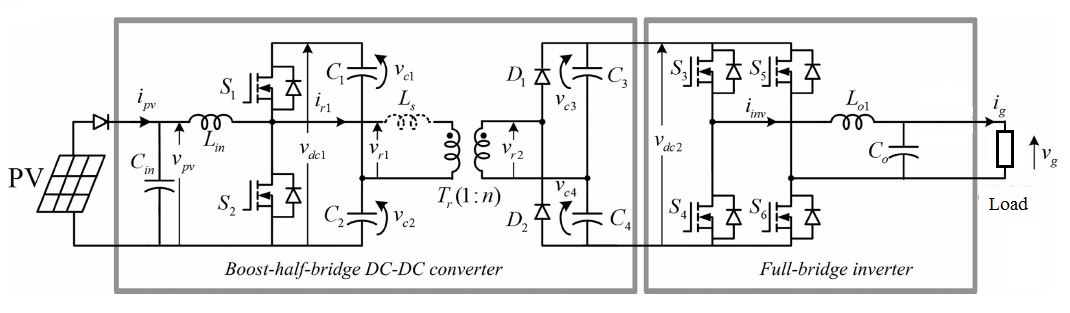
\includegraphics[width= 14 cm]{ct.jpg}
%\caption{ System Circuit Diagram}
%\end{figure}
%%%%%%%%%%%%%%%%%%%%%%%%%%%%%%%%%%%

\section{Motivation for this work}

The identification of many medicinal plants often requires an expert, and there is a shortage of such experts in India. Furthermore, the conversion of rural lands and forests into commercial developments has an adverse impact on the number of medicinal plants that may be threatened. Safeguarding medicinal plants requires a concrete knowledge of the availability and spread of such plants across India, and how commercial development is affecting the survival and availability of medicinal plants. One specific aspect of this would involve the design and development of an automated medicinal plant identification system.




\section{Methodologies Adopted}

In this project, we use deep learning algorithms to solve the problem. There are many deep learning algorithms that can be applied. We’ll be using three deep learning algorithms in our project. The algorithms are:
\begin{itemize}
\item{Deep Neural Network}
\item{Convolutional Neural Network}
\item{Transfer Image Learning}
\end{itemize}
These algorithms are implemented and evaluated and the one which gives the optimal results will be selected to be implemented in the Android application. 


\section{Outline of the Report}

This report contains 4 chapters. Chapter 1 gives the introduction to the project work and describes the objectives of the work. Literature survey is described in Chapter 2. System Design is explained in the Chapter 3. Methodology is well explained in chapters 4 . The report concludes with a chapter describing the future development and scope.


\chapter{LITERATURE REVIEW}
Many recent studies exist on plant classification and identification based on different plant features. However, to handle such features information, finding an efficient classification method has become an area of active study.
Many researchers have attempted and worked very much in this area. Most papers propose and use Machine Learning techniques to tackle the problem. Some researchers have proposed the use of Deep Learning techniques such as Artificial Neural Networks. Many have achieved great accuracies with their models. But most of these papers are only research and their results are inaccessible or unavailable for use by the general public.

\section{Identification of Philippine Herbal Medicine Plant Leaf Using Artificial Neural Network}
[1] By Robert G. de Luna, Renann G. Baldovino, Ezekiel A. Cotoco,
Anton Louise P. de Ocampo, Ira C. Valenzuela, Alvin B. Culaba, Elmer P. Dadios

\paragraph{}
The study described in this paper consists of a system
that involves image processing techniques to extract relevant
features related to leaf in conjunction with using artificial neural
network in order to detect and identify some Philippine herbal
plants. Real samples of twelve different herbal medicine plant
leaves are collected where each leaf are isolated in single image.
Several features are extracted using techniques in image
processing. With the artificial neural network acting as an
autonomous brain network, the system can identify the species of
the herbal medicine plant leaves being tested. The system can also
provide information about the diseases the herbal plant can be used to cure.

For the training, a features dataset of 600 images coming from
50 images per herbal plant are used. With the aid of Python, a
neural network model with optimized parameters is established
producing 98.16\% identification for the whole dataset. To evaluate
the actual performance of the system, a separate 72 sample images
of herbal plants are tested with the neural network model
implemented in MATLAB. Experimental results demonstrate a
98.61\% accuracy of herbal plant identification.\\

In the system, the researchers provided a program that will
serve as the tool for the user in order to distinguish specific
herbal medicine plant leaves, with the aid of a camera installed
along with the system to capture image of a leaf specimen. The
captured image will be processed and analyzed using different
techniques of image processing in order to obtain defined
parameters. Around 20 to 30 features
are used for recognition of plant. For this study, several
primary features will be used to obtain around 5 secondary
features that will serve the purpose of identification.

They developed a computer program that has the ability to
learn from examples and can thus also perform recognition of
previously unseen patterns. A supervised multilayer perceptron
(MLP) artificial neural network (ANN) will be used in this
system. Training is carried out by presenting a succession of
data records (the training set) to the network, each record
containing data from a specimen or record of known identity.\\

The resultant ability of the network to recognize previously
unseen patterns is periodically tested using an independent
"validation" dataset, also containing data records of known
classes. After identification, necessary display of
result is presented. In this proposed work, experimental
analysis was carried out with 12 herbal plant species approved
by the Department of health (DOH) for medical applications.
Fifty leaves were taken from each plant
species and clustered.

\section{Leaves Classification Using Neural Network Based on Ensemble Features }
[2] By Sigit Adinugroho, Yuita Arum Sari
\paragraph{}
An automated plant identification is necessary to identify plants, especially rarely seen ones. In this paper a framework to identify plant species based on leaf's characteristics is introduced. First, 31 features of leaves from 13 species are extracted that represents color, shape and texture of the leaves. Then, the features are selected according to their correlation to the class label. The data with 25.8\% pruned features are then used to train a feedforward neural network. The network is trained and tested using 975 images by implementing 10-fold mechanism yielding 95.54\% accuracy.

This paper implements leaf-based plant recognition using
ensemble features based on texture, color, and shape. Those
features are used to recognize a plant using neural network
classifier. Their main contribution is in determining
appropriate features as well as selection of optimum parameters
in neural network classifier. This research uses a publicly available leaves dataset
named Swedish leaf dataset. The dataset contains 1125
Swedish tree leaf images from 15 species, with 75 images
per species. This research focuses primarily on simple leaves.
Their system consists of the phases: Segmentation, Feature Extraction, Feature Selection, Neural Network Training and Testing

This research uses 31 features extracted from three basic
characteristics of a leaf: Shape, Color, and Texture. In order to reduce the number of neural network’s input nodes
which leads to reducing training and testing time, the
importance of each feature is measured. To do that, Pearson
correlation coefficient is calculated to assess how well a
feature and the class label correlates.\\

Feedforward neural network (FFNN) is a type of neural network which
has three types of layers: input layer, hidden layers and output
layer. Each node in a layer is connected to each node in the
following layer without any feedback connection.
This experiment makes use of an FFNN with single layer
of input, hidden, and output nodes. The number of nodes in
the input layer depends on the number of features from the
input data, while the number of nodes in the hidden layer
is also tested to find most effective number. On
the other hand, the number of nodes in output layer is always
13 that is equal to the number of the class in the dataset. 

It is shown that the accuracy increases as more are
features added. However, the accuracy converges to values
around 80\% starting from 13 features. Adding more
features does not significantly increase the accuracy. The
maximum accuracy is 84\% achieved by 23 features. In other
words, the feature selection is able to reduce 25.8\% of the
features. The maximum accuracy is 95.54\%
with 14 hidden nodes. This paper proposes an approach for plant
recognition based on leaf characteristics. Feature selection has
managed to reduce the number of features by 25.8\%.
Experiment result from the dataset indicates that the method
has a promising result shown by the accuracy of 95.54\% by
using 14 hidden nodes.


\section{Identification of Ayurvedic Medicinal Plants by Image Processing of Leaf Samples }
[3] By Manojkumar P., Surya C. M., Varun P. Gopi
\paragraph{}
Colour and texture from both sides of the leaf contain
deterministic parameters to identify the species. This paper
explores feature vectors from both the front and back side of
a green leaf along with morphological features to arrive at a
unique optimum combination of features that maximizes the
identification rate. A database of medicinal plant leaves is created
from scanned images of front and back side of leaves of commonly
used ayurvedic medicinal plants. The leaves are classified based
on the unique feature combination. Identification rates up to
99\% have been obtained when tested over a wide spectrum
of classifiers. The above work has been extended to include
identification by dry leaves and a combination of feature vectors
is obtained, using which, identification rates exceeding 94\% have
been achieved.

A set of medicinal plant leaf images were collected from a private botanical
garden. 20 leaves were collected in a random manner from
40 different plant species used for Ayurvedic, herbal and folk
medicines. The leaves were collected from their natural habitat
and the selection of leaves and plants were quite random. The
leaves were spread out on an ordinary document scanner and
scanned with highest possible resolution. Both the front and
back sides were scanned and the images were stored in jpeg
format for further processing.\\

Initially 131 features are extracted from the front and back
side of each leaf image. This set includes 36 centroid-radii
(CR) distances, 12 geometrical features,
24 colour features, 40 texture features, 7 HU
invariant moments and 12 Zernike moments.
These features are extracted from each of the 20 leaves
belonging to 40 species.

In this proposed method, 800 and 400 samples are taken
for training and testing respectively. Different combinations
of feature vectors are tested using MLP and SVM to assess the performance. Highest
identification rate (ID rate) of 99\% is obtained in MLP
using Geometric-Colour-Texture-Zernike combination with 38
features, followed closely by Geometric-Colour-Texture combination with 30 features with an ID rate of 98.7\%. In SVM,
maximum ID rate of 98.8\% is for Geometric-Colour-Texture-Zernike combination with 38 features followed by 98.1\% for
CR-Geometric-colour-Texture combination having 48 features.
From the results it can be concluded that Geometric-Colour-Texture-Zernike combination results in highest classification
rate in MLP classifier and may be employed in the problem
of identifying medicinal plants from samples of green leaves
if the requirement is to maximize ID Rate.\\

In this proposed method, 800 and 400 samples are taken
for training and testing respectively. Colour features cannot
be employed for identifying plants using dry leaves. Texture
features gets distorted when the leaves dry and we cannot
depend on these two features for plant identification problem.
Extraction of venation features is quite challenging from dry
leaves. Geometric, centroid-radii, HU invariant moments and
Zernike moments may, however be employed effectively for
the dry leaf. In this paper total 37 features were extracted from
dry leaf.

The effectiveness of individual feature sets along with their
combinations are then analysed using SVM and MLP classifiers to find the optimum combination, which is then tested
with different classifiers. Different classifiers were used to
identify the plants using dry leaves. Among this MLP yields
highest ID rate of 94.5\%.

\section{Plant Species Identification Based on Neural Network}
[4] By Lei Zhang, Jun Kong, Xiaoyun Zeng, Jiayue Ren
\paragraph{}
Aided Plant Species Identification acts
significantly on plant digital museum system and
systematic botany, which is the groundwork for research
and development of plant. This paper presents a new
method for plant species identification using leaf image. It
focuses on the stable features extraction of leaf, such as
the geometrical features of shape and the texture features
of venation. The 2-D moment invariants, Wavelet
statistical features are used to extract leaf information.
Self-Organizing Feature Map (SOM) neural network has
the advantages of simple structure, ordered mapping
topology and low complexity of learning. It is suitable for
many complex problems such as multi-class pattern
recognition, high dimension input vector and large
quantity training data. So this paper uses SOM neural
network to identify the plant species. The experimental
results illustrate the effectiveness of this method.

In this paper, the geometrical feature
and the texture feature are all extracted and used for plant
species identification.
The plant species identification system is operated in
two phases: the training and the
identification. In the training phase the leaves samples of
known plant species are provided to the system. By
feature extracting, the produced feature values are used to
train the SOM neural network. In the identification phase,
query plant leaf image passes through the feature
extraction to obtain a set of feature values, which are
input to the trained SOM artificial neural network, the
trained SOM neural network will give decision of the
query plant species.\\

\noindent The system contains several modules,
which are described below:
\begin{enumerate}
	\item{Leaf image acquisition and preprocessing}
	\item{Feature extraction:}
	\begin{itemize}
		\item{Geometry feature can
		be computed by 2-D moment invariants and the ratio of
		leaf length to width, secondly the texture feature is
		extracted by multi-resolution Gabor filters and statistical
		moments.\\}
	\end{itemize}
	\item{Identification}
	\begin{itemize}
		\item{The feature values of known plant
		species are used to train the SOM neural network. And
		the trained SOM neural network can be used to identify
		the query leaf sample\\}
	\end{itemize}
\end{enumerate}

In this paper, a plant identification method based on
SOM neural network is proposed and performed. Firstly,
the shape feature of the leaf is extracted by 2-D moment
invariants and approximately ratio. Secondly, the Discrete
Wavelet Transform and statistical moments are employed
to capture the texture information of nervation. Finally,
the SOM neural network is used to identify the species of
the plant. Experimental results reveal this method is
feasible and effective in some plant species identification.
As the next step, they plan to involve in studying and implementing plant species
identification in the complex background and
illumination.  


\chapter{SYSTEM DESIGN}

System design is the process of designing the elements of a system such as the architecture, modules and components, the different interfaces of those components and the data that goes through that system.

\section{System Architecture}
\begin{figure}[h]
	\label{ss}
	\centering
	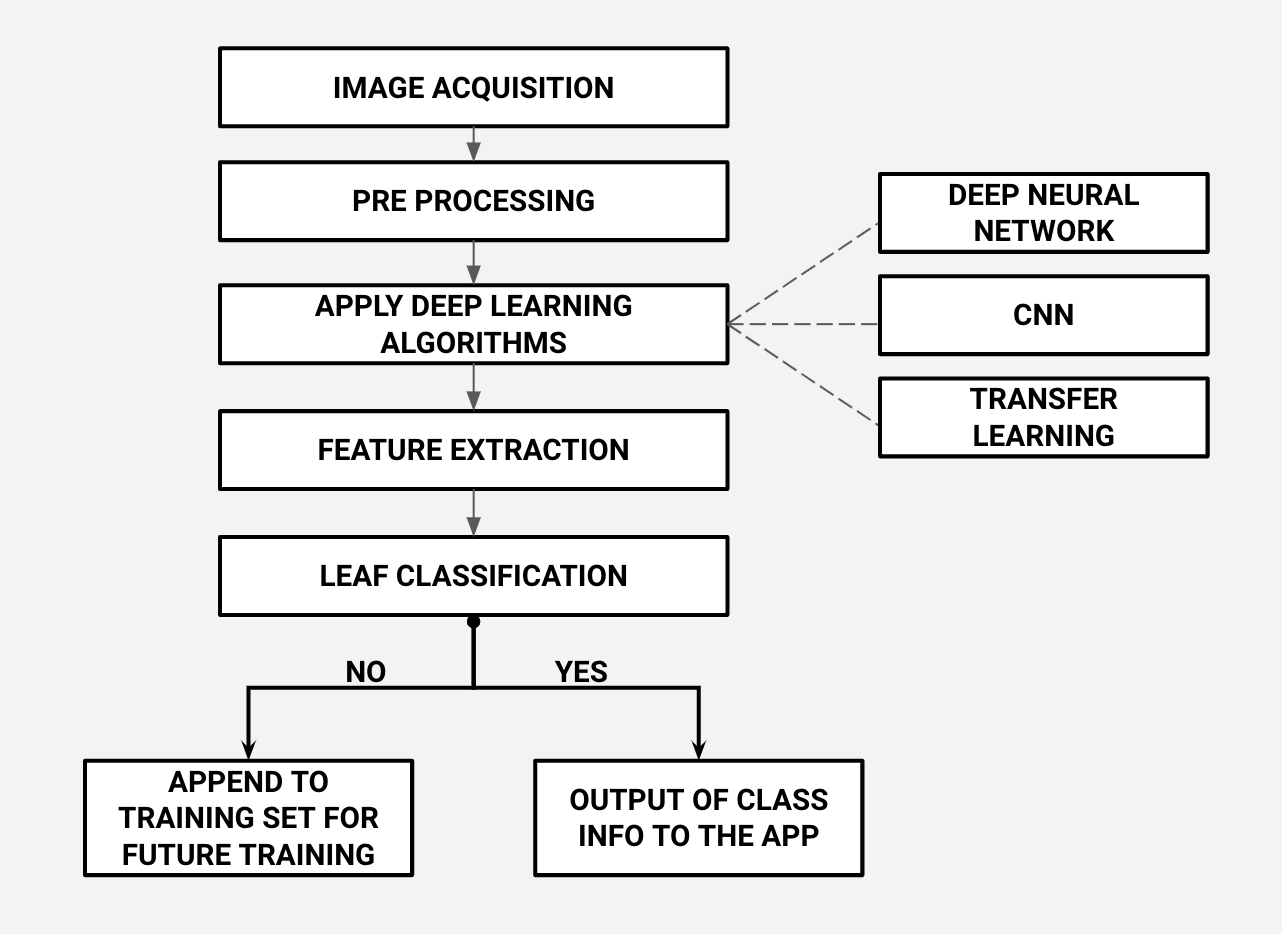
\includegraphics[width= 15.8 cm]{waterfall.png}
	\caption{System Architecture}
\end{figure}
The proposed system identifies the Ayurvedic plant with an image of its leaf taken using an android application.
User captures image of the leaf of the Ayurvedic plant to be identified.
App uses deep learning model to identify the class of the leaf and displays result. The major steps involved in identification are:\\
\begin{itemize}
 \item Image Acquisition
 \item  Preprocessing
 \item Apply Deep Learning Algorithms
 \item  Feature Extraction
 \item Leaf Classification
\end{itemize}


\subsection{Image Acquisition }
The images of the leaf of the plant is captured using an android application.
\subsection{Preprocessing}
The image taken is first preprocessed in the system. Some of the various preprocessing techniques applied are
\begin{itemize}
    \item{Uniform Aspect Ratio}\\One of the first steps is to ensure that the images have the same size and aspect ratio. Most of the neural network models assume a square shape input image, which means that each image needs to be checked if it is a square or not, and cropped appropriately. Cropping can be done to select a square part of the image.
    \item{Image Scaling}\\Once we have ensured that all images are square (or have some predetermined aspect ratio), it’s time to scale each image appropriately. 
    \item{Dimensionality Reduction}\\We could choose to collapse the RGB channels into a single gray-scale channel.
\end{itemize}
\subsection{Apply Deep Learning Algorithms}
Deep learning is a type of machine learning (ML) and artificial intelligence (AI) that imitates the way humans gain certain types of knowledge. It teaches the computer to learn by example.\\
Three different Deep Learning techniques are used to tackle the problem.
\begin{itemize}
    \item Deep Neural Network
    \item Convolutional Neural Network (CNN)
    \item Transfer Learning
\end{itemize}
\subsubsection{Deep Neural Network}
Deep Neural Networks mainly involves neural networks.
The structure of a neural network is like any other kind of network there is an interconnected web of nodes, which are called neurons,and the edges that join them together.A neural network's main function is to receive a set of inputs perform progressively complex calculations and then use the output to solve a problem.
\subsubsection{Convolutional Neural Networks}
It's essentially a Neural Network that uses convolution in place of general matrix multiplication in one of their layers.
CNN uses some features of the visual cortex.
CNN has the special ability to determine patterns in an image.
It takes in an input image, assign learnable weights and biases to various aspects/objects in the image and be able to differentiate one from the other.
\subsubsection{Transfer Learning}
Transfer learning make use of the knowledge gained while solving one problem and applying it to a different but related problem. It's an optimization in general.\\
In transfer learning, we first train a base network on a base dataset and task, and then we transfer them, to a second network to be trained on another dataset and task. This process will tend to work if the features are general, meaning suitable to both base and target tasks.\\ \\
Performance of these three Deep Learning techniques is analysed and evaluated and the one with the best accuracy is taken.
\subsection{Stages in Deep Learning }
60 classes of medicinal plants with 1000 samples per class is used in the system.
The stages in the system are:- \\
\begin{itemize}
    \item {Training Stage:}
       In this stage the Leaf images are preprocessed and the Deep Learning models learn the features from images. 
       Trained models can now be used for identifying test samples.
    \item {Validation Stage:}
       Images from the training set are used to test the trained model.
    \item{Testing Stage:}
       The test leaf samples ie. the images of the leaves are used to test the model. 
\end{itemize}
\begin{table}
\begin{center}
\begin{tabular}{ |p{1.5cm}|p{5cm}|p{5cm}| }
 \hline
 \multicolumn{3}{|c|}{Ayurvedic Plant Leaves} \\
 \hline
 Sl No: &Local Name &Botanical Name\\
 \hline
 1   & Indian Elm    &Holoptelea Integrifolia\\
 2   & Willow-leaved justicia    &Justicia Beddomei\\
 3   & Chabakam    &Michelia Champaca\\
 4   & Adapathiyan    &Holostemma Ada- Kodien\\
 5   &Aromatic Ginger  &Kaempferia Galanga\\
 6   & Spanish Cherry   &Mimusops Elendig\\
 7   & Chethi  &Ixora Coccinea\\
 8   & Air Plant  &Kalanchoe Pinnata\\
 9   & Curry leaf tree   &Muraya Koenigii (Linn)\\
 10  & Licorice Weed   &Scoparia Dulcis\\
 11  & Nutmeg    &Myristica Fragrans\\
 12  & Malabar Plum   &Syzygium Jambos\\
 13  & Scarlet Leadwort  &Plumbago Indica\\
 14  & Canton Ginger  &Zingiber Officinale\\
 15  & Common Gauva &Psidium Guajava\\
 16  & Chini    &Acalypha Fruticosa\\
 17  & Cinnamon    &Cinnamomum Zeylanicum\\
 18  & Aloe vera   &Aloe Vera\\
 19  & Screw tree    &Helicterus Isora\\
 20  & Sodom Apple    &Calotropis Procera\\

 \hline
\end{tabular}
\end{center}
\caption{Some plants in the database}
\end{table}


\chapter{METHODOLOGY}

The purpose of project methodology is to allow for controlling the entire management process through effective decision making and problem solving, while ensuring the success of specific processes, approaches, techniques, methods and technologies.

\section{Deep Neural Network }
\paragraph{}
The structure of a deep neural network is like any other kind of network. There is an interconnected web of nodes, which are called neurons and the edges that join them together. A neural network's main function is to receive a set of inputs, perform progressively complex calculations, and then use the output to solve a problem.
Neural nets are used for classification tasks where an object can fall into one of at least two different categories. A deep neural network is highly structured and comes in layers. The first layer is the input layer, the final layer is the output layer, and all layers in between are referred to as hidden layers.
\begin{figure}[h]
	\label{ss}
	\centering
	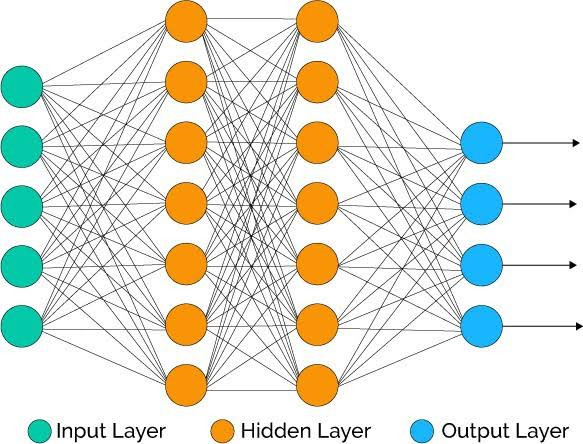
\includegraphics[width= 9 cm]{neural.jpg}
	\caption{Deep Neural Network}
\end{figure}
A neural net can be viewed as the result of spinning classifiers together in a layered web.
This is because each node in the hidden and output layers has its own classifier. A set of inputs is passed to the first hidden layer, the activations from that layer are passed to the next layer and so on until you reach the output layer, where the results of the classification are determined by the scores at each node. This happens for each set of inputs.
This series of events starting from the input where each activation is sent to the next layer,
and then the next, all the way to the output, is known as forward propagation or forward prop.


Forward propagation is a neural net's way of classifying a set of inputs. Each node has the same classifier, and none of them fire randomly. If you repeat an input, you get the same output. Each edge has a unique weight, and each node has a unique bias. This means that the combination used for each activation is also unique, which explains why the nodes fire differently. The prediction accuracy of a neural net depends on its weights and biases. We want that accuracy to be high, meaning we want the neural net to predict a value that is as close to the actual output as possible, every single time.

The process of improving a neural net’s accuracy is called training, just like with other machine learning methods. To train the neural network, the output from forward propagation is compared to the output that is known to be correct, and the cost is the difference between the two.The point of training is to make that cost as small as possible, across millions of training examples. To do this, the network tweaks the weights and biases step by step
until the prediction closely matches the correct output.Once trained well, a deep neural net has the potential to make accurate predictions each time.This is a deep neural net in a nutshell.


\section{CNN (Convolutional Neural Network) }
\paragraph{}
CNN (Convolutional Neural Network) is so influential that they’ve made Deep Learning one of the hottest topics in AI today. CNNs were pioneered by Yann Lecun of New York University, who also serves as the director of Facebook's AI group. It is currently believed that Facebook uses a CNN for its facial recognition software. A convolutional net has been the go-to solution for machine vision projects in the last few years. Early in 2015, after a series of breakthroughs by Microsoft, Google, and Baidu, a machine was able to beat a human at an object recognition challenge for the first time in the history of AI. It’s hard to mention a CNN without touching on the ImageNet challenge. ImageNet is a project that was inspired by the growing need for high-quality data in the image processing space
\paragraph{}
In neural networks, Convolutional Neural Network (ConvNets or CNNs) is one of the main techniques to perform image recognition and image classification. Objects detection, face recognition, etc. are some of the areas where CNNs are widely used.
CNN-based image classifiers take an input image, process it and classify it under certain categories (Eg., Dog, Cat, Tiger, Lion). Computers sees an input image as an array of pixels and it depends on the image resolution. Based on the image resolution, it will see h x w x d ( h = Height, w = Width, d = Dimension ).
\subsection{Layers in CNN}
There are many component layers in CNN:-

A typical deep CNN has four sets of layers:-
\begin{itemize}
\item{Convolutional Layer}
\item{ReLu Activation}
\item{Pooling Layer}
\item{Fully Connected Layer}
\end{itemize}

\subsubsection{Convolution Layer}
Convolution is the first layer to extract features from an input image. Convolution preserves the relationship between pixels by learning image features using small squares of input data. It is a mathematical operation that takes two inputs such as image matrix and a filter or kernel.
\begin{figure}[h]
	\label{ss}
	\centering
	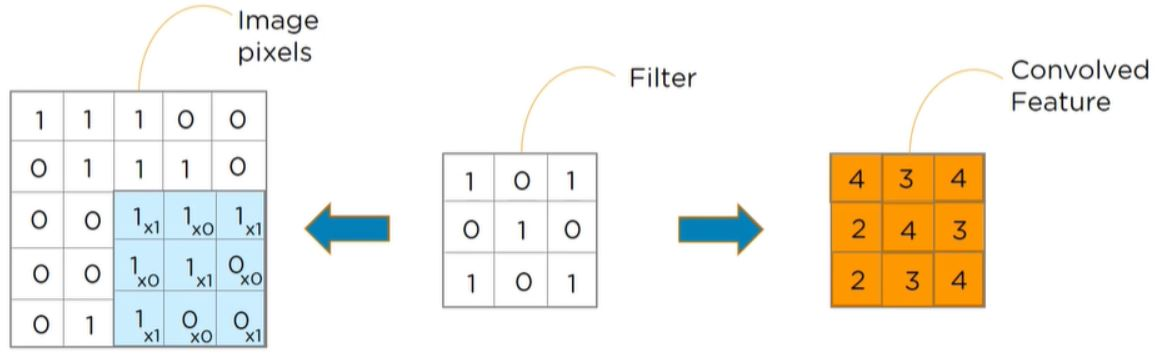
\includegraphics[width= 13 cm]{convolutionlayer.jpg}
	\caption{Convolution Process}
\end{figure}

Convolution of an image with different filters can perform operations such as edge detection, blur and sharpen by applying filters.
Consider a 5x5 whose image pixel values are 0, 1 and filter matrix 3x3. Then the convolution process is done in which a 5x5 image matrix is multiplied with the 3x3 filter matrix which is called “Feature Map”.
The matrix filter is slid over the pixels of the image and the dot product is computed which forms the convolved feature map.

\subsubsection{ReLu Activation}
ReLu activation function is applied to the convolution layer to get a rectified feature map.
Each node in the convolutional layer is connected to a node that fires like in other nets. The activation used is called ReLu, or Rectified Linear Unit. CNNs are trained using backpropagation, so the vanishing gradient is once again a potential issue. For reasons that depend on the mathematical definition of ReLu, the gradient is held more or less constant at every layer of the net. So the ReLu activation allows the network to be properly trained, without harmful slowdowns in the crucial early layers. The ReLu activation function finally gives a rectified feature map.

\subsubsection{Pooling}
The pooling layer is used for dimensionality reduction. CNNs tile multiple instances of
convolutional layers and ReLu layers together in a sequence, in order to build more and
more complex patterns. The problem with this is that the number of possible patterns becomes exceedingly large. By introducing pooling layers, we ensure that the net focuses on only the most relevant patterns discovered by convolution and ReLu. This helps limit
both the memory and processing requirements for running a CNN. The Pooling layer is responsible for reducing the spatial size of the convolved feature. This is to decrease the computational power required to process the data through dimensionality reduction. \\
\begin{figure}[h]
	\label{ss}
	\centering
	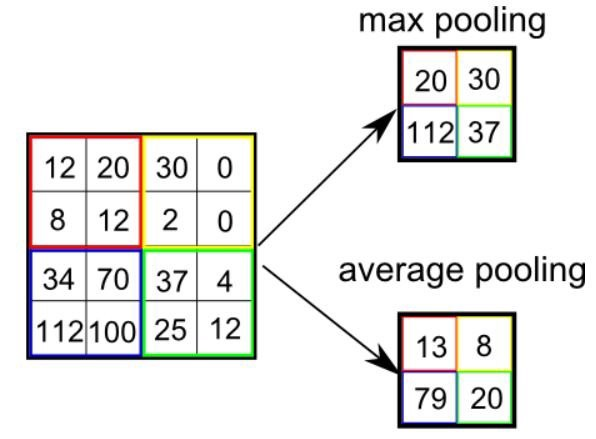
\includegraphics[width= 9 cm]{pooling1.jpg}
	\caption{Pooling}
\end{figure}

There are two types of Pooling:
\begin{itemize}
\item{Max Pooling}
\item{Average Pooling}
\end{itemize}


Max Pooling returns the maximum value from the portion of the image covered by the Kernel. On the other hand, Average Pooling returns the average of all the values from the portion of the image covered by the Kernel.


\subsubsection{Fully Connected Layer}
Together, these three layers can discover a host of complex patterns, but the neural network will
have no understanding of what these patterns mean. 
In the layer we call as the FC layer, we flatten our matrix into a vector and feed it into a fully connected layer like a neural network. So a fully connected layer is attached
to the end of the network in order to equip the network with the ability to classify data samples.
With the fully connected layers, we combine these features together to create a model. Finally, we have an activation function such as softmax or sigmoid to classify the outputs into any of the output class labels.
\begin{figure}[h]
	\label{ss}
	\centering
	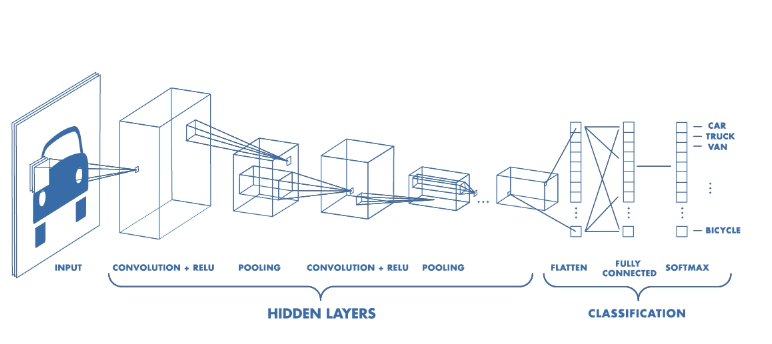
\includegraphics[width= 16 cm]{CNN.png}
	\caption{Convolutional Neural Network}
\end{figure}
\paragraph{}
Since CNNs are such deep networks, they most likely need to be trained using
server resources with GPUs. Despite the power of CNNs, these networks have one drawback. Since they are a supervised
learning method, they require a large set of labeled data for training, which can be
challenging to obtain in a real-world application.

\section{Transfer Image Learning}
Transfer learning is popular in Deep learning given the enormous resources required to train deep learning models or the large and challenging datasets on which deep learning models are trained.\\
In transfer learning, we first train a base network on a base dataset and task, and then we transfer them, to a second network to be trained on another dataset and task. This process will tend to work if the features are general, meaning suitable to both base and target tasks.\\
The benefits of Transfer Learning are that it can speed up the time it takes to develop
and train a model by reusing these pieces or modules of already developed models. This
helps speed up the model training process and accelerate results.
Transfer learning make use of the knowledge gained while solving one problem and applying it to a different but related problem.
\subsection{Transfer Learning Approaches}
Two common approaches are as follows:
\begin{itemize}
    \item Develop Model Approach
    \item Pre-trained Model Approach
\end{itemize}
\subsubsection{Develop Model Approach}
\textbf{Select Source Task}\\ You must select a related predictive modeling problem with an abundance of data where there is some relationship in the input data, output data, and/or concepts learned during the mapping from input to output data.\\
\textbf{Develop Source Model}\\ Next, you must develop a skillful model for this first task. The model must be better than a naive model to ensure that some feature learning has been performed.\\
\textbf{Reuse Model}\\ The model fit on the source task can then be used as the starting point for a model on the second task of interest. This may involve using all or parts of the model, depending on the modeling technique used.\\
\textbf{Tune Model}\\ Optionally, the model may need to be adapted or refined on the input-output pair data available for the task of interest.\\
\subsubsection{Pre-trained Model Approach}
\textbf{Select Source Model}\\ A pre-trained source model is chosen from available models. Many research institutions release models on large and challenging datasets that may be included in the pool of candidate models from which to choose from. \\
\textbf{Reuse Model}\\ The model pre-trained model can then be used as the starting point for a model on the second task of interest. This may involve using all or parts of the model, depending on the modeling technique used. \\
\textbf{Tune Model}\\ Optionally, the model may need to be adapted or refined on the input-output pair data available for the task of interest.\\
This second type of transfer learning is common in the field of deep learning. \\
\subsection{Transfer Learning with Image Data}
It is common to use a deep learning model pre-trained for a large and challenging image classification task be used for other similar tasks.
These models can be downloaded and incorporated directly into new models that expect image data as input.
Three examples of models of this type includes
\begin{itemize}
    \item Oxford VGG Model
    \item Google Inception Model
    \item Microsoft ResNet Model
\end{itemize}
Transfer learning is an optimization, a shortcut to saving time or getting better performance.
In general, it is not obvious that there will be a benefit to using transfer learning in the domain until after the model has been developed and evaluated.
\subsection{Conditions to use Transfer Learning}
There are three possible benefits to look for when using transfer learning:\\[0.3cm]
\textbf{Higher start}\\ The initial skill (before refining the model) on the source model is higher than it otherwise would be.\\
\textbf{Higher slope}\\ The rate of improvement of skill during training of the source model is steeper than it otherwise would be.\\
\textbf{Higher Asymptote}\\ The converged skill of the trained model is better than it otherwise would be.\\

Ideally, you would see all three benefits from a successful application of transfer learning.\\
It is an approach to try if you can identify a related task with abundant data and you have the resources to develop a model for that task and reuse it on your own problem, or there is a pre-trained model available that you can use as a starting point for your own model. \\
On some problems where you may not have very much data, transfer learning can enable you to develop skillful models that you simply could not develop in the absence of transfer learning.


\begin{figure}[h]
	\label{ss}
	\centering
	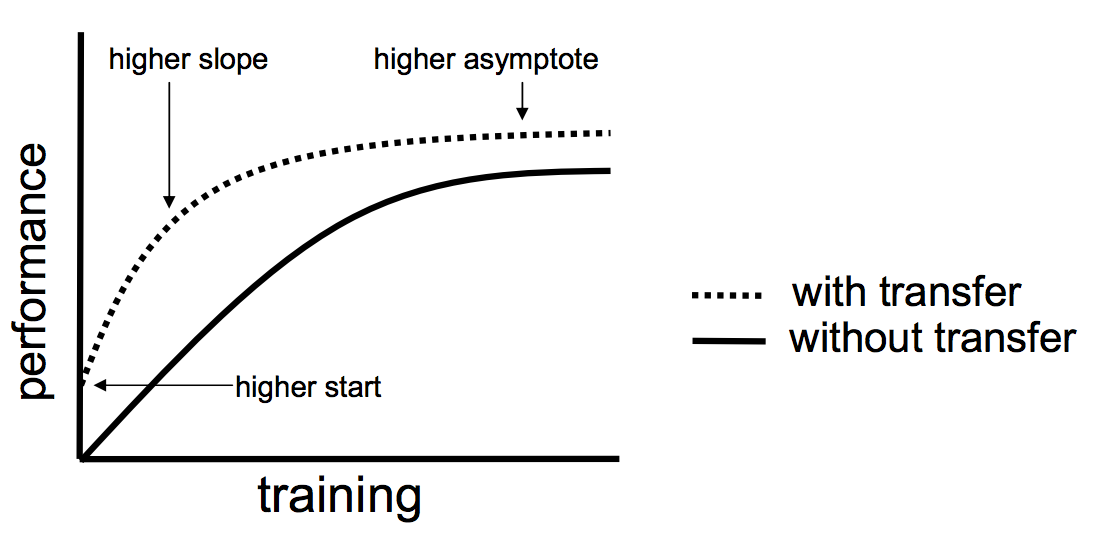
\includegraphics[width= 16 cm]{transfer.png}
	\caption{Three ways in which transfer might improve learning.}
\end{figure}

\section{VGG19}
AlexNet was released in 2012 and it improved on the traditional Convolutional Neural Networks. VGG can be considered as a successor of the AlexNet. It was created by a group called Visual Geometry Group at University of Oxford and hence the name VGG. The VGG network architecture was introduced by Simonyan and Zisserman in their 2014 paper, \emph{Very Deep Convolutional Networks for Large Scale Image Recognition}. It carries and uses some ideas from it's predecessors and improves on them and uses deep Convolutional neural layers to improve accuracy.\\\\
VGG19 is a variant of VGG model which consists of 19 layers: 16 Convolution layers, 3 Fully Connected layers, 5 Max Pool layers and 1 Softmax layer. There are other variants of VGG like VGG11, VGG16 and others. VGG19 has 19.6 billion FLOPs.\pagebreak

\subsection{Layers}
This network is characterized by its simplicity, using only 3×3 convolutional layers stacked on top of each other in increasing depth. Reducing volume size is handled by max pooling. Two fully-connected layers, each with 4,096 nodes are then followed by a softmax classifier.\\\\
A summary of the layers in the VGG19 model can be found in the following image:\\

\begin{figure}[h]
	\label{ss}
	\centering
	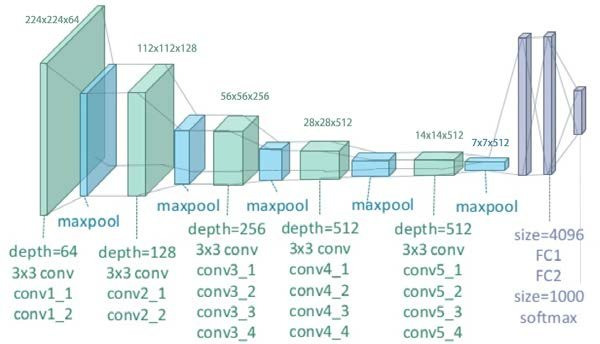
\includegraphics[width= 16 cm]{vgg19-layers.png}
	\caption{Layers in VGG19}
\end{figure}
\pagebreak
The table in the figure below contains the details of number of filters, parameters and activations for each layer in the VGG19 model:\\

\begin{figure}[H]
	\label{ss}
	\centering
	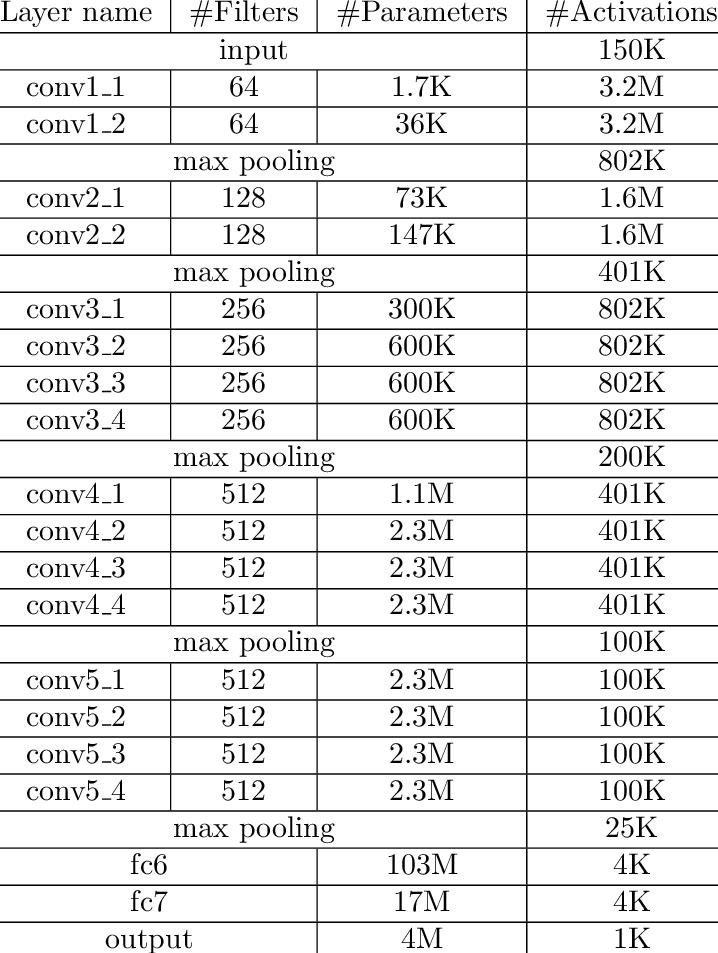
\includegraphics[width=20cm,height=15cm,keepaspectratio]{vgg19-arch-details.png}
	\caption{Details on the VGG19 layers}
\end{figure}

\subsection{Architecture}
A fixed size of (224 * 224) RGB image was given as input to this network. So the input matrix was of shape (224,224,3).
The only preprocessing that was done is that the mean RGB value is subtracted from each pixel, over the whole training set.
Kernels of (3 * 3) size with a stride size of 1 pixel were used. This enabled to cover the whole notion of the image.
Spatial padding was used to preserve the spatial resolution of the image.
Max pooling was performed over a 2 * 2 pixel windows with a stride of 2.
This was followed by Rectified linear unit(ReLu) to introduce non-linearity to make the model classify better and to improve computational time.
Three fully connected layers were implemented from which first two were of size 4096 and followed by a layer with 1000 channels for 1000-way ILSVRC classification and the final layer is a softmax function.

\subsection{Results}
On a single test scale, VGG achieved a top-1 error of 25.5\% and a top-5 error of 8.0\%. At multiple test scales, VGG got a top-1 error of 24.8\% and a top-5 error of 7.5\%. VGG also achieved second place in the 2014 ImageNet competition with its top-5 error of 7.3\%, which was decreased to 6.8\% after the submission.

\subsection{Usages}
\begin{itemize}
    \item Considered to be one of the best vision model architectures
    \item Used as a great classification architecture for many different datasets
    \item Weights are easily available with frameworks like Keras
    \item Transfer Learning
\end{itemize}


\chapter{IMPLEMENTATION AND DEPLOYMENT}

\section{Software Requirements}
These are main sofware requirements to implement the proposed solution.

\subsection{NumPy}
NumPy is a general-purpose array-processing package.  It is a Python library that provides a multidimensional array object, various derived objects (such as masked arrays and matrices), and an assortment of routines for fast operations on arrays, including mathematical, logical, shape manipulation, sorting, selecting, I/O, discrete Fourier transforms, basic linear algebra, basic statistical operations, random simulation and much more.  At the core of the NumPy package, is the ndarray object.  This encapsulates n-dimensional arrays of homogeneous data types, with many operations being performed in compiled code for performance.

\subsection{TensorFlow}
TensorFlow is an open-source software library released in 2015 by Google to make it easier for developers to design, build, and train deep learning models. TensorFlow is available on different operating systems such as Linux, Windows, macOS, and also on mobile operating platforms like iOS and Android.  One of the salient features of TensorFlow is that it is capable of running on multiple CPUs and GPUs.  The computations in Tensor-Flow are reported as stateful dataflow graphs. TensorFlow is considered the first serious implementation of a framework focused on deep learning. TensorFlow can train and run deep neural networks for handwritten digit classification, image recognition, word embeddings, recurrent neural networks, sequence-to-sequence models for machine translation, natural language processing, and PDE (partial differential equation) based simulations. TensorFlow supports production prediction at scale, with the same models used for training.

\subsection{Keras}
Keras is a high-level neural networks API, written in Python and capable of running on top of TensorFlow, CNTK, or Theano. It was developed with a focus on enabling fast experimentation. It focuses on being user-friendly, modular, and extensible. It was developed as part of the research effort of project ONEIROS (Open-ended Neuro-Electronic Intelligent Robot Operating System). Keras contains numerous implementations of commonly used neural-network building blocks such as layers, objectives, activation functions, optimizers, and a host of tools to make working with image and text data easier.

In addition to standard neural networks, Keras has support for convolutional and re-current  neural  networks.   It  supports  other  common  utility  layers  like  dropout,  batchnormalization, and pooling.

Keras allows users to productize deep models on smartphones (iOS and Android), on the web, or on the Java Virtual Machine. It also allows use of distributed training of deep-learning models on clusters of Graphics Processing Units (GPU) and Tensor processingunits (TPU).

\subsection{TensorFlow Lite}
TensorFlow Lite is TensorFlow’s lightweight solution for mobile and embedded devices. It lets you run machine-learned models on mobile devices with low latency. Classification, regression, or anything else you might want without necessarily incurring a round trip to a server. It’s presently supported on Android and iOS via a C++ API, as well as having a Java Wrapper for Android Developers. TensorFlow Lite is a set of tools to help developers run TensorFlow models on mobile, embedded, and IoT devices. It enables on-device machine learning inference with low latency and a small binary size. TensorFlow Lite is designed to make it easy to perform machine learning on devices, "at the edge" of the network, instead of sending data back and forth from a server.

\subsection{Android Studio}
Android Studio is the official IDE for Android app development, based on IntelliJ IDEA. On top of IntelliJ’s powerful code editor and developer tools, Android Studio offers even more features that enhance your productivity when building Android apps, such as a flexible Gradle-based build system, a fast and feature-rich emulator, a unified environment where you can develop for all Android devices, Instant Run to push changes to your running app without building a new APK, etc.


\chapter{CONCLUSION}
\paragraph{}
We have used a dataset of images of 55 Ayurvedic species of leaves to train and develop deep learning models that can identify Ayurvedic leaves from outside world with good prediction. We used three deep learning techniques viz.  Deep Neural Network, Convolutional Neural Network, and Transfer Learning and inferred that Transfer Learning gave the best results. We deployed the model that gave the best results in an Android application and it produces inferences on real world leaves with good accuracy and inference time.

\section{Scope}
Ayurveda and herbal medicines are greatly used and followed worldwide, especially in India. Herbal medicine plants pose a big impact on the health of every people around the world.  But the major issue we face is difficulty in efficiently and effectively identifying the plants that form the ingredients for the medicine.
This application can be used by users from any background to identify ayurvedic medicinal plants by capturing images or videos of the same.
Thus we believe this work is a major step forward in the efficient and effective identification of Ayurvedic medicinal plants and also provides a good reference for future works in this field.

\section{Future Developments}
We shall add more species of leaves into the dataset and let the model learn from them too so that users can use the application to identify more species. The application only identifies and outputs the name of the identified plant species along with it's common name for now. We shall add a feature either to display further details and medicinal uses of the identified species in the app itself if the user chooses, or add links that take the users to resources available online that contain such details about the identified species. We shall also add more features based on user feedback.


%%%%%%%%%%%%%%%%%%%%%%%%%%%%%%%%%%%%
%%%%%%%%%%%%%%%%%%%%%%%%%%%%%%%%%%%%
%%
%%          Bibliography 
%%
%%%%%%%%%%%%%%%%%%%%%%%%%%%%%%%%%%%%
%%%%%%%%%%%%%%%%%%%%%%%%%%%%%%%%%%%%

\clearpage
\addcontentsline{toc}{chapter}{\quad BIBLIOGRAPHY}
\begin{thebibliography}{99}

\bibitem{a}
Identification of Philippine Herbal Medicine Plant Leaf Using Artificial Neural Network Robert G. de Luna, Renann G. Baldovino, Ezekiel A. Cotoco, Anton Louise P. de Ocampo, Ira C. Valenzuela, Alvin B. Culaba, Elmer P. Dadios Gokongwei College of Engineering, De La Salle University Manila, Philippines

\bibitem{b}
Leaves Classification Using Neural Network Based on Ensemble Features, Sigit Adinugroho, Yuita Arum Sari

\bibitem{c}
Identification of Ayurvedic Medicinal Plants by Image Processing of Leaf Samples,Manoj kumar P., Surya C. M., Varun P. Gopi, 2017 Third International Conference on Research in Computational Intelligence.

\bibitem{d}
Plant Species Identification Based on Neural Network, Lei Zhang, Jun Kong, Xiaoyun Zeng, Jiayue Ren

\bibitem{e}
Identification of Selected Medicinal Plant Leaves Using Image Features and ANN, R.Janani, A.Gopal

\bibitem{f}
Plant Recognition System Based on Neural Networks, W.H.Rankothge , D.M.S.B Dissanayake, U.V.K.T Gunathilaka, S.A.C.M Gunarathna, C.M Mudalige

\bibitem{g}
Leaf Features based approach for Automated Identification of Medicinal Plants, E. Sandeep Kumar and Viswanath Talasila,International Conference on Communication and Signal Processing, April 3-5, 2014, India

\bibitem{h}
Leaf Recognition and Classification Algorithm to be used by Indigenous Medicine, Madhuka G . P . D Udantha, Ayola D.N Jayamaha, 2014 International Conference on Advances in ICt for Emerging Regions

\bibitem{i}
Zhong-Qiu Zhao, Peng Zheng, Shou-tao Xu, and Xindong Wu, Object Detection with Deep Learning: A Review

\bibitem{j}
Ross Girshick, Je Donahue, Trevor Darrell, and Jitendra Malik. Rich feature hierarchies for accurate object detection and semantic segmentation.

\bibitem{k}
Joseph Redmon, Santosh Divvala, Ross Girshick, and Ali Farhadi. You only look once:Unified, real-time object detection. International Conference on Advances in ICt for Emerging Regions

\bibitem{l}
Abdul Kadir, Lukito Edi Nugroho, Adhi Susanto, and Paulus Insap
Santosa, “Leaf classi¿cation using shape, color, and texture features,”
arXiv preprint arXiv:1401.4447, 2013.

\bibitem{m}
https://www.analyticsvidhya.com/blog/2017/09/understaing-support-vector- machine-example-code/

\bibitem{n}
https://en.wikipedia.org/wiki/Transfer\_learning

\bibitem{o}
https://en.wikipedia.org/wiki/Deep\_learning

\bibitem{p}
https://en.wikipedia.org/wiki/Support-vector\_machine

\bibitem{q}
https://en.wikipedia.org/wiki/Convolutional\_neural\_network

\bibitem{r}
https://en.wikipedia.org/wiki/Multilayer\_perceptron

\end{thebibliography}



%%%%%%%%%%%%%%%%%%%%%%%%%%%%%%%%%%%%%
%%%%%%%%%%%%%%%%%%%%%%%%%%%%%%%%%%%%%
\clearpage



%%%%%%%%%%%%%%%%%%%%%%%%%%%%%%%%%%%%%
%%%%%%%%%%%%%%%%%%%%%%%%%%%%%%%%%%%%%
%%%%%%%%%%%%%%%%%%%%%%%%%%%%%%%%%%%%%
%%%%%%%%%%%%%%%%%%%%%%%%%%%%%%%%%%%%%


%%%%%%%%%%%%%%%%%%%%%%%%%%%%%%%%%%%%%
%%%%%%%%%%%%%%%%%%%%%%%%%%%%%%%%%%%%%
%
%   Hi, All
%   Arun Xavier, VAST Thrissur
%
%   for more  Visit my Page - http://arunxeee.blogspot.in/
%
%%%%%%%%%%%%%%%%%%%%%%%%%%%%%%%%%%%%
%%%%%%%%%%%%%%%%%%%%%%%%%%%%%%%%%%%%

%
\end{spacing}
\newpage
\thispagestyle{empty}
\vspace*{\fill}
\begin{flushright}

\includegraphics[width=2.5 cm]{VidyaLogo.JPG}\\[.2 cm]
{\Large \bf \rm  Department of \vdept\ }\\
{\large \rm Vidya Academy of Science \& Technology\\
Thalakkottukara, Thrissur - 680 501\\
({\tt http://www.vidyaacademy.ac.in})}
\end{flushright}

%
\end{document}



%%%%%%	Any Problems Contact me  @  arunxeee.blogspot.com
%%%%%								      aruncx@gmail.com
%%%%%%%%%%%%%%%%
%%%%
%%%%
%%%%%%%%%%%
%%
%